\documentclass{jarticle}
\usepackage{myarticle}
\usepackage[dvipdfmx]{graphicx}

\title{一様乱数を使う}
\author{渡辺 宙志}
\affiliation{慶応義塾大学理工学部物理情報工学科}
\abst{
一様乱数からさまざまな確率密度関数に従う確率変数を表現する方法を紹介する。
}

\newcommand{\diff}{{\mathrm d}}

\begin{document}

\maketitle

\section{確率変数と確率密度}

ある数列$x_n$を考えよう。いま、$x_1, x_2, \cdots, x_n$まで値が定まっているとき、
次の値$x_{n+1}$が確率的に決まるような変数を確率変数と呼ぶ。
また、それまでの値$x_1, x_2, \cdots, x_n$と$x_{n+1}$が全く無関係である場合、
この数を乱数と呼ぶ。サイコロを10回振って出た目の履歴と、11回目に出る目は
無関係であるので乱数であると言える。

確率変数$X$が連続変数であるとしよう。また、簡単のため、定義域が有界で、$0 \le X \le 1$でる場合のみを考える。
確率変数$X$が値$x$から$x+\diff x$までの値をとる確率が
\begin{equation}
P(x \le X < x +\diff x) = f(x) \diff x \label{eq_density}
\end{equation}
とあらわされるとき、関数$f(x)$を$X$の{\bf 確率密度関数 (probability density function, PDF)}と呼ぶ\footnote{確率空間の定義についてはより厳密な定義が望ましいが、ここでは深入りしない。}。
ただし、関数$f(x)$は規格化条件
\begin{equation}
\int_0^1 f(x) \diff x  = 1 
\end{equation}
を満たす。
この式を
\begin{equation} \label{eq_density2}
P(X = x) = f(x)
\end{equation}
などと表現、理解しないようにしよう。式(\ref{eq_density2})は
「確率変数$X$が、値$x$を持つ確率は$f(x)$であらわされる」という意味で、
式(\ref{eq_density})より理解しやすいかもしれない。
サイコロなど、離散変数の場合はこれでも良いが、
連続変数$X$がピンポイントで何かの値$x$を持つという事象の確率はゼロである。
厳密な議論については測度論を参照することにして、今は、式(\ref{eq_density})が定義だと覚えておけば問題はない。

さて、式(\ref{eq_density})は微分の形をしており、このままでは扱いにくい。
そこで、$X$が$x$以下の値をとる確率$P(0\le X < x)$を考える。
これは式(\ref{eq_density})を積分することで得られ、
\begin{eqnarray}
P(0\le X < x) &=& \int_0^x \diff x f(x)\\
&=& F(x) \label{eq_cdf}
\end{eqnarray}
とあらわされる。この関数$F(x)$を、{\bf 累積密度関数 (cumulative 
distribution function, CDF)}と呼ぶ。

確率密度関数が定数である場合、つまり確率変数$X$が、ある範囲$x \le  X < x + \diff x$を取る確率が
$x$に依存しない場合、この確率変数を一様乱数であるという。定義域が$0\le X<1$であるような一様乱数の
確率密度関数は$f(x) = 1$である。この一様乱数に従う確率変数を$R$としよう。
一様乱数$R$から、なんらかの変換$g(R) = X$により、任意の確率密度関数$f(x)$に従う確率変数$X$を作るのが本稿の目的である。

さて、一様乱数の定義から、確率変数$R$が、値$0 \le  R < r$を取る確率は
\begin{equation}
P(0 \le  R < r ) \equiv \int_0^r \diff r = r
\end{equation}
である。これと式(\ref{eq_cdf})を見比べれば、
$F(X) = R$という変数変換をすると、一様乱数$R$から確率密度関数$f(x)$に従う確率変数$X$ができることがわかる。
実際、$F(X) = R$という変換で作られた確率変数$X$が、$0  \le X < x$という範囲の値を取る確率は
\begin{equation}
P(0 \le  X < x ) = P(0 \le  R < F(x)) = F(x)
\end{equation}
であることから\footnote{変数変換$F(X) = R$のもとでは、$X=x$であるとき、$R=F(x)$である。}、
\begin{equation}
P(x \le  X < x + \diff x ) = f(x)\diff x
\end{equation}
であり、確かに確率密度関数$f(x)$に従っていることがわかる。
つまり、一様乱数から任意の確率密度関数に従う確率変数を作るには、「確率密度関数の原始関数の逆関数」を用いて変数変換をすれば良いことがわかる。直感的な説明は図\ref{fig_xrmap}を参照のこと。

\begin{figure}
\begin{center}
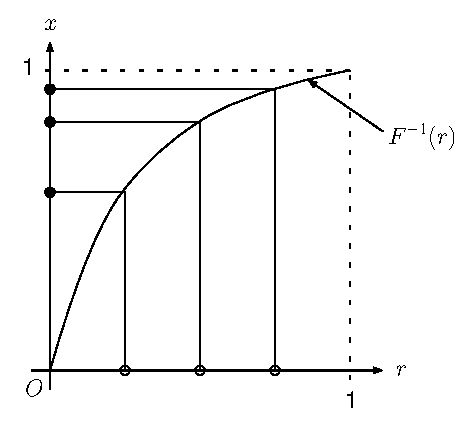
\includegraphics[width=.50\linewidth]{xrmap.eps}
\caption{
一様乱数$r$から確率密度$f(x)$であるような確率変数$X$を生成する方法は
図のように写像として理解できる。
一様に並んだ点(図の白丸)を、ある関数を使って$x$軸上に移動することを考える。
このとき、うつされた点(図の黒丸)の{\bf 密度}が$f(x)$となるように
変換しなければならない。したがって$0 \le x \le x'$までの点の数は、
$f(x')$の原始関数$F(x')$である。
したがって、その逆関数$F^{-1}(r)$を使って$r$を変換すればよいことがわかる。
図では$f(x) = x$であるような場合を例示してある。このとき$F^{-1}(r) = r^{1/2}$となる。
}
\label{fig_xrmap}
\end{center}

\end{figure}

\section{有界の定義域の場合}

まず、確率変数$X$の定義域が有限である場合について
いくつか例を挙げよう。簡単のため、$X$のとりうる値は$[0,1]$であるとする。

\subsection{一様乱数}

$X$が一様変数であるとしよう。このとき$f(x)=1$であるから、その積分は
$F(x)=x$となる。その逆関数も$F^{-1}(x)=x$であるから、結局
$g(r)=r$、すなわち、生成された一様乱数$r$をそのまま使えばよい。

\subsection{密度が線形の場合}
\label{sec_linear}

$f(x)=x$であるような確率変数$X$を再現したいとする。
これは、$0 \le X \le 1$の範囲で、出る値が、値自身に比例するような
変数である。たとえば、十分小さな$\Delta x$について
$0.1 < x < 0.1 + \Delta x $の範囲の値をとる確率は
$0.01 < x < 0.01 + \Delta x $の10倍となる。

このとき、$F(x)=x^2$であるので、逆関数は$g(r) = F^{-1}(r) = r^{1/2}$となる。
すなわち、生成された一様乱数の平方根を使えば、このような確率変数を
再現することができる。

\subsection{単位円内に一様分布する点}

単位円の中に一様に点をばらまくことを考える。これは
条件$x^2+y^2 \le 1$を満たすような座標$(x,y)$をランダムに生成することに対応する。
極座標$x = r \cos \theta, y = r \sin \theta $を使って表現すると、
角度は一様であるから、$\theta$に関しては
単に$0 \le \theta < 2\pi$であるような一様乱数を使えばよい。
動径方向$r$に関しては、一様乱数を使ってしまうと円の中心付近になるほど
密度が高くなるような分布になってしまうので、ちゃんと考えなくてはいけない。

この場合、まず$f(x)$がどうなっているか考える。$f(x)$は、
半径$x < r < x + \Delta x$にある点の数に対応する。したがって、
$F(x)$は、半径$x$の円の中の点の数、要するに面積であるから、$x^2$に比例する。
これは\ref{sec_linear}節の場合と同じであるから、$r$として一様乱数の平方根を使えばよい。
以上をまとめると、$[0,1]$上の一様乱数 $r$と、$[0,2\pi]$上の一様乱数$\theta$を使って、
\begin{eqnarray}
x &=& r^{1/2} \cos \theta \\
y &=& r^{1/2} \sin \theta 
\end{eqnarray}
とすればよい。


\subsection{単位球面に一様分布する点}

単位球の表面に一様に点をばらまくには少し工夫がいる。
単位球の表面は、極座標 $(\theta,\phi)$で表すことができるが、
$(\theta,\phi)$に対して、ヤコビアンが $\sin \theta \diff \theta \diff \phi$で
あったことを思い出そう。このままでは、$\sin \theta$に比例するように
$\theta$を生成しなければならない。
ここで変数変換
\begin{equation}
z = \cos \theta
\end{equation}
を施せば、
\begin{equation}
\diff z = -\sin \theta \diff \theta
\end{equation}
となるので、ヤコビアンは $-\diff z \diff \phi$となる。
したがって2変数$(z,\phi)$で表現すれば、$z$、$\phi$ともに
一様乱数でよい。具体的には、$[-1,1]$上の一様乱数$z$及び、$[0,2\pi]$上の一様乱数$\phi$を
用いて、
\begin{eqnarray}
x &=& \sqrt{1-z^2} \cos \phi \\
y &=& \sqrt{1-z^2} \sin \phi\\
z &=& z 
\end{eqnarray}
とすれば、球面上に一様に分布する点$(x,y,z)$が得られる\footnote{
ここでは変数変換という形を取ったが、
やっていることは $f(\theta) = \sin \theta$であるような確率変数$\theta$を
$F^{-1}(z)$を使って一様乱数$z$から表現することと等価である。
$F(\theta) = \cos \theta$であるから、一様乱数$z$を用いて
$\theta = \cos^{-1} z$とすればよい。これより$z = \cos \theta$である。
}。

\subsection{単位球内に一様分布する点}

単位球内に一様に点をばらまくには、単位球面の場合にに加えて動径方向の分布を
考えてやればよい。\ref{sec_linear}節の場合と同様に考えれば、一様乱数$r~(0\le r \le 1)$を使って、
\begin{eqnarray}
x &=& r^{1/3} \sqrt{1-z^2} \cos \phi \\
y &=& r^{1/3} \sqrt{1-z^2} \sin \phi\\
z &=& r^{1/3} z 
\end{eqnarray}
とすれば、球内に一様に分布する点$(x,y,z)$が得られる。

\section{定義域が有界でない場合}

\subsection{原子崩壊(指数分布)}

定義域が有界でない場合も同様に計算することができる。
たとえば、一個の放射性元素を考えよう。
単位時間あたり$\lambda$の確率で崩壊するとき、この元素が
崩壊するまでの時間$T$は確率変数となるが、
それはどのように表現できるだろうか。
単位時間あたりの崩壊確率$\lambda$は崩壊定数と呼ばれ、このような確率過程は
パラメータ$\lambda$の指数分布に従うことがわかっている。

この時、時間$t$までに崩壊する確率は
\begin{equation}
P(0 \le T < t) = 1 - \mathrm{e}^{-\lambda t} \equiv F(t)
\end{equation}
で表される。従って、一様乱数$R$から$T$を作るには、
\begin{eqnarray}
1 - \mathrm{e}^{-\lambda T} = R
\end{eqnarray}
を$T$について解いて、
\begin{eqnarray}
T = - \frac{\ln (1-R)}{\lambda}
\end{eqnarray}
とすれば良い。

\subsection{正規乱数}

定義域が有界でない例で重要なのは、正規乱数と呼ばれる乱数である。
この乱数は、発生頻度が標準正規分布(すなわち、平均が$0$、分散が$1$のガウス分布)
であるような乱数である。
一様乱数から正規乱数を発生させる方法はいくつかあるが、
ここでは{\bf ボックス・ミューラー(Box-Muller)法}を紹介する。
範囲が$(0,1)$であるような二つの独立な一様乱数$r_1, r_2$を用意する。
この乱数を用いて、独立な正規化された乱数$x_1, x_2$は
\begin{equation}
\begin{array}{l}
x_1 = \sqrt{-2\ln r_1} \cos 2\pi r_2\\
x_2 = \sqrt{-2\ln r_1} \sin 2\pi r_2
\end{array} \label{eq_bm}
\end{equation}
であらわすことができる。詳しい証明や理由は省くが、おおまかに説明すると、
$x_1$、$x_2$が独立で標準正規分布に従う時、
$\sqrt{x_1^2+x_2^2}$はレイリー分布に従うことがわかる。
そこで、一様乱数からレイリー分布を発生させ、$x_1$、$x_2$について解けば
式(\ref{eq_bm})を得る。

\end{document}

